\documentclass[mathserif]{beamer}
\usetheme{Antibes}

\setbeamertemplate{items}[circle]
\setbeamertemplate{bibliography item}{\insertbiblabel}

\usepackage{xeCJK}
\setCJKmainfont{新細明體}

\usepackage{caption}
\captionsetup{font=scriptsize,labelfont=scriptsize}
\setlength\belowcaptionskip{-1pt}

\usepackage{amsmath,amssymb,amsfonts}
\DeclareMathOperator*{\divby}{/}
\DeclareMathOperator*{\maxi}{max}
\DeclareMathOperator*{\avg}{avg}
\DeclareMathOperator*{\where}{|}

\newcommand\expfigvspace{-2.5ex}

\usepackage{graphicx}
\usepackage{tablefootnote}
\usepackage{subcaption}

\usepackage{array}
\usepackage{multirow}
\usepackage{tablefootnote}


\title{From CopeOpi Scores to CopeOpi Vectors:\\Word Vectors for Multi-class Text Classification}
\author{
	Pei-Shan Tsai\\
	{\small Advisor: Ying-ping Chen}
}
\institute{
	Natural Computing Laboratory\\
	Department of Computer Science\\
	National Chiao Tung University
}
\date{2017}


\AtBeginSubsection[]
{
  \begin{frame}
    \frametitle{Table of Contents}
    \tableofcontents[ 
		currentsubsection,
		hideothersubsections, 
		sectionstyle=show/hide, 
		subsectionstyle=show/shaded/hide,
		subsubsectionstyle=show/show/hide,
		] 

  \end{frame}
}

\begin{document}
\frame{\titlepage}

\begin{frame}{Table of Contents}
	\tableofcontents[ 
		sectionstyle=show/show, 
		subsectionstyle=hide,
		subsubsectionstyle=hide,
		] 
\end{frame}


\section{The Text Classification Problems}
\subsection{The Text Classification Problems}
\subsubsection{Background}
\begin{frame}{Background}
\begin{itemize}
\item Millions of digital texts are generated everyday. To derive useful information from these digital texts, text
mining has become a popular area of both research and business
	\begin{itemize}
	\item Text classification is one of the most important task
	\end{itemize}
\item \alert{Text classification}, or text categorization
	\begin{itemize}
	\item Assigning a document to a set of predefined classes, categories or labels
	\end{itemize}
\item In the past, text classification problems were solved by
	\begin{itemize}
	\item Manually assignment
	\item Knowledge engineering approaches (hand-crafted classification rules)
	\item Both are expensive to scale due to the needs of skilled labors and expert knowledge
	\end{itemize}
\item Nowadays, works on classification focus on \alert{machine learning approaches}
\end{itemize}
\end{frame}

\subsubsection{Definition}
\begin{frame}{Definition of Text Classification}
\begin{block}{Definition (Text Classification)}
In a text classification problem, we are given
	\begin{itemize}
	\item A document space $\mathbb{X}$
	\item A set of predefined classes $\mathbb{C}$
	\end{itemize}
The task of text classification can be defined as an unknown assignment function
	\begin{equation*}
	f: \mathbb{X} \times \mathbb{C} \rightarrow \{\mathtt{True},\mathtt{False}\}
	\end{equation*}
which assigns each pair $\langle d,c \rangle \in \mathbb{X} \times \mathbb{C}$ a Boolean value $\mathtt{True}$ if the document $d$ is in the class $c$ or $\mathtt{False}$ otherwise\cite{Feldman2006tm,Manning2008tm}
\end{block}
\end{frame}

\begin{frame}{Definition of Supervised Learning for Text Classification}
\begin{block}{Definition (Supervised Learning for Text Classification)}
By using
	\begin{itemize}
	\item A machine learning algorithm $\Gamma$
	\item A labeled training set $\mathbb{D}=\{\langle d,c \rangle \where \langle d,c \rangle \in \mathbb{X} \times \mathbb{C}\}$
	\end{itemize}
We wish to learn a \alert{classifier}, or classification function $\gamma$ which approximates the unknown assignment function $f$ as close as possible\cite{Sebastiani2002mltm,Feldman2006tm,Manning2008tm}
	\begin{equation*}
	\begin{gathered}
	\Gamma(\mathbb{D}) = \gamma \\
	\gamma: \mathbb{X} \times \mathbb{C} \rightarrow \{\mathtt{True},\mathtt{False}\} \approx f
	\end{gathered}
	\end{equation*}
\end{block}
\end{frame}

\subsubsection{Applications}
\begin{frame}{Applications}
Typically, the document space $\mathbb{X}$ can be any kinds of texts and the classes $\mathbb{C}$ are defined for the user needs, thus text classification has a wide variety of applications in text mining
\begin{itemize}
\item Document organization and information retrieval
	\begin{itemize}
	\item $\mathbb{X}$ = articles
	\item $\mathbb{C}$ = topics
	\end{itemize}
\item Sentiment analysis and opinion mining
	\begin{itemize}
	\item $\mathbb{X}$ = customer reviews
	\item $\mathbb{C}$ = positive, negative
	\end{itemize}
\item Email routing and spam filtering
	\begin{itemize}
	\item $\mathbb{X}$ = emails
	\item $\mathbb{C}$ = spam, not-spam
	\end{itemize}
\end{itemize}
\end{frame}

\section{Vector Space Models}


\subsection{Different Types of Frequency Matrix}

\begin{frame}{The Vector Space Models}
	\begin{itemize}
	\item To teach machines to understand our languages, we need to design a representation which they can manipulate
	\item Vector space model (VSM) is an algebraic model for \alert{representing texts as vectors}
		\begin{itemize}
		\item Based on a series of statistical semantics hypothesis: takes event frequencies in corpora as clues to discover latent semantic
		\item Derived vectors from a \alert{frequency matrix}
			\begin{itemize}
			\item The structure of the matrix relates to the scope of application of the vector space model\cite{Turney2010vsm}
			\end{itemize}	
		\end{itemize}
	\end{itemize}
\end{frame}

\subsubsection{Similarity of Documents: The Term-Document Matrix}
\begin{frame}{Similarity of Documents: The Term-Document Matrix}
\begin{block}{Hypothesis (Bag-of-words Hypothesis)}
The frequencies of words in a document tend to indicate the relevance of the document to a query\cite{Salton1975vsmh1}.
\end{block}
If documents and queries have similar column vectors in a term-document matrix, then they tend to have similar meanings.\\
\scalebox{0.7}{
\begin{tabular}{cccccc}
                       &                               & \multicolumn{4}{c}{Documents}                                                                                             \\
                       &                               & $d_1$                               & $d_2$                               & $\cdots$              &                       \\ \cline{3-6} 
\multirow{3}{*}{Terms} & \multicolumn{1}{c|}{$t_1$}    & \multicolumn{1}{c|}{$f{d_1}_{t_1}$} & \multicolumn{1}{c|}{$f{d_2}_{t_1}$} & \multicolumn{1}{c|}{} & \multicolumn{1}{c|}{} \\ \cline{3-6} 
                       & \multicolumn{1}{c|}{$t_2$}    & \multicolumn{1}{c|}{$f{d_1}_{t_2}$} & \multicolumn{1}{c|}{$f{d_2}_{t_2}$} & \multicolumn{1}{c|}{} & \multicolumn{1}{c|}{} \\ \cline{3-6} 
                       & \multicolumn{1}{c|}{$\vdots$} & \multicolumn{1}{c|}{}               & \multicolumn{1}{c|}{}               & \multicolumn{1}{c|}{} & \multicolumn{1}{c|}{} \\ \cline{3-6} 
\multicolumn{1}{l}{}   & \multicolumn{1}{l|}{}         & \multicolumn{1}{l|}{}               & \multicolumn{1}{l|}{}               & \multicolumn{1}{l|}{} & \multicolumn{1}{l|}{} \\ \cline{3-6} 
\end{tabular}}
\end{frame}

\subsubsection{Similarity of Words: The Word-Context Matrix}
\begin{frame}{Similarity of Words: The Word-Context Matrix}
\begin{block}{Hypothesis (Distributional Hypothesis)}
Words that occur in similar contexts tend to have similar meanings\cite{Harris1954vsmh2,Firth1957vsmh2}.
\end{block}
If words have similar row vectors in a word-context matrix, then they tend to have similar meanings.\\
\scalebox{0.7}{
\begin{tabular}{cccccc}
                       &                               & \multicolumn{4}{c}{Contexts}                                                                                              \\
                       &                               & $c_1$                               & $c_2$                               & $\cdots$              &                       \\ \cline{3-6} 
\multirow{3}{*}{Words} & \multicolumn{1}{c|}{$w_1$}    & \multicolumn{1}{c|}{$f{c_1}_{w_1}$} & \multicolumn{1}{c|}{$f{c_2}_{w_1}$} & \multicolumn{1}{c|}{} & \multicolumn{1}{c|}{} \\ \cline{3-6} 
                       & \multicolumn{1}{c|}{$w_2$}    & \multicolumn{1}{c|}{$f{c_1}_{w_2}$} & \multicolumn{1}{c|}{$f{c_2}_{w_2}$} & \multicolumn{1}{c|}{} & \multicolumn{1}{c|}{} \\ \cline{3-6} 
                       & \multicolumn{1}{c|}{$\vdots$} & \multicolumn{1}{c|}{}               & \multicolumn{1}{c|}{}               & \multicolumn{1}{c|}{} & \multicolumn{1}{c|}{} \\ \cline{3-6} 
\multicolumn{1}{l}{}   & \multicolumn{1}{l|}{}         & \multicolumn{1}{l|}{}               & \multicolumn{1}{l|}{}               & \multicolumn{1}{l|}{} & \multicolumn{1}{l|}{} \\ \cline{3-6} 
\end{tabular}}
\end{frame}

\subsubsection{Similarity of Relations: The Pair-Pattern Matrix}
\begin{frame}[shrink=10]{Similarity of Relations: The Pair-Pattern Matrix}
\begin{block}{Hypothesis (Extended Distributional Hypothesis)}
Patterns co-occurring with similar word-pairs tend to have similar meanings\cite{Lin2001vsmh3}.
\end{block}
If patterns have similar column vectors in a pair-pattern matrix, then they tend to express similar semantic relations.
\begin{block}{Hypothesis (Latent Relation Hypothesis)}
Word-pairs co-occurring in similar patterns tend to have similar semantic relations\cite{Turney2003vsmh4}.
\end{block}
If word-pairs have similar row vectors in a pair-pattern matrix, then they tend to have similar semantic relations.\\
\scalebox{0.7}{
\begin{tabular}{cccccc}
                            &                                             & \multicolumn{4}{c}{Patterns}                                                                                                                                \\
                            &                                             & $p_1$                                                & $p_2$                                                & $\cdots$              &                       \\ \cline{3-6} 
\multirow{3}{*}{Word-pairs} & \multicolumn{1}{c|}{$(w_1^a\text{:}w_1^b)$} & \multicolumn{1}{c|}{$f{p_1}_{(w_1^a\text{:}w_1^b)}$} & \multicolumn{1}{c|}{$f{p_2}_{(w_1^a\text{:}w_1^b)}$} & \multicolumn{1}{c|}{} & \multicolumn{1}{c|}{} \\ \cline{3-6} 
                            & \multicolumn{1}{c|}{$(w_2^a\text{:}w_2^b)$} & \multicolumn{1}{c|}{$f{p_1}_{(w_2^a\text{:}w_2^b)}$} & \multicolumn{1}{c|}{$f{p_2}_{(w_2^a\text{:}w_2^b)}$} & \multicolumn{1}{c|}{} & \multicolumn{1}{c|}{} \\ \cline{3-6} 
                            & \multicolumn{1}{c|}{$\vdots$}               & \multicolumn{1}{c|}{}                                & \multicolumn{1}{c|}{}                                & \multicolumn{1}{c|}{} & \multicolumn{1}{c|}{} \\ \cline{3-6} 
\multicolumn{1}{l}{}        & \multicolumn{1}{l|}{}                       & \multicolumn{1}{l|}{}                                & \multicolumn{1}{l|}{}                                & \multicolumn{1}{l|}{} & \multicolumn{1}{l|}{} \\ \cline{3-6} 
\end{tabular}}
\end{frame}

\subsection{Construction of Vector Space Models}
\begin{frame}{Construction of Vector Space Models}
	\begin{itemize}
	\item Linguistic Processing
		\begin{itemize}
		\item Tokenization
		\item Normalization
		\item Annotation
		\end{itemize}
	\item Mathematical Processing\cite{Lowe2001}
		\begin{itemize}
		\item Building the frequency matrix
		\item Weighting the elements
		\item Dimensionality reduction
		\item Comparing the similarities
		\end{itemize}
	\end{itemize}
\end{frame}


\section{From CopeOpi Scores to CopeOpi Vectors}
\subsection{CopeOpi Scores}
\subsubsection{What are CopeOpi scores?}
\begin{frame}
\frametitle{What are CopeOpi scores?}
\begin{itemize}
\item Sentiment scores of Chinese characters/words\cite{Ku2007score}
	\begin{itemize}
	\item Sentiment polarities: positive/negative
	\item Strength of sentiment polarities
	\item $+1$(positive) $\sim$ $-1$(negative)
	\end{itemize}
\item The meaning of a Chinese word\\$=f(\text{the meanings of its composite characters})$
\item The sentiment of a Chinese word\\$=f(\text{sentiments of its composite characters})$
\end{itemize}
\end{frame}
\subsubsection{How to compute CopeOpi scores?}
\begin{frame}
\frametitle{How to compute CopeOpi scores?}
\begin{itemize}
\item How to get the sentiment score of a Chinese character?
	\begin{itemize}
	\item Assume that
		\begin{itemize}
		\item Characters in a positive opinion word tend to be positive
		\item Characters in a negative opinion word tend to be negative
		\end{itemize}
	\end{itemize}
\item The observation probabilities of a character in positive and negative opinion words
	\begin{itemize}
	\item NTUSD (NTU Sentiment Dictionary)\cite{Ku2007ntusd} as seed words
	\end{itemize}
\end{itemize}
\end{frame}
\subsubsection{The computation scheme of CopeOpi scores}
\begin{frame}
\frametitle{The computation scheme of CopeOpi scores}
\begin{block}{Computation Scheme (CopeOpi Scores)}
Given two corpora
\begin{itemize}
\item $\mathbb{W}_p=\{\text{Chinese positive opinion words}\}$
	\begin{itemize}
	\item the vocabulary $\mathbb{V}_p=\{\text{unique characters in }\mathbb{W}_p\}$
	\end{itemize}
\item $\mathbb{W}_n=\{\text{Chinese negative opinion words}\}$
	\begin{itemize}
	\item the vocabulary $\mathbb{V}_n=\{\text{unique characters in }\mathbb{W}_n\}$
	\end{itemize}
\end{itemize}
For each character $c_i \in \mathbb{V}_p \cup \mathbb{V}_n$, we can compute its CopeOpi score $\mathcal{COP}_{c_i}$
\end{block}
\end{frame}

\begin{frame}
\frametitle{The computation scheme of CopeOpi scores}
\begin{block}{Computation Scheme (CopeOpi Scores)}
The CopeOpi score $\mathcal{COP}_{c_i}$ of a character $c_i$
\begin{equation*}
\begin{gathered}
\mathcal{P}_{c_i} = \dfrac {
	fp_{c_i} \divby \sum_{c \in \mathbb{V}_p} fp_c
}{
	fp_{c_i} \divby \sum_{c \in \mathbb{V}_p} fp_c +
	fn_{c_i} \divby \sum_{c \in \mathbb{V}_n} fn_c
}
\\
\mathcal{N}_{c_i} = \dfrac {
	fn_{c_i} \divby \sum_{c \in \mathbb{V}_n} fn_c
}{
	fp_{c_i} \divby \sum_{c \in \mathbb{V}_p} fp_c +
	fn_{c_i} \divby \sum_{c \in \mathbb{V}_n} fn_c
}
\\
\mathcal{COP}_{c_i} = \mathcal{P}_{c_i} - \mathcal{N}_{c_i}
\end{gathered}
\end{equation*}
\end{block}
\begin{flushright}
\vspace{-9.5ex}
\scalebox{0.7}{
\begin{tabular}{rp{0.5cm}p{0.5cm}}
& $\mathbb{W}_p$ & $\mathbb{W}_n$\\ \cline{2-3} 
\multicolumn{1}{l|}{$c_i$} & \multicolumn{1}{l|}{$fp_{c_i}$} & \multicolumn{1}{l|}{$fn_{c_i}$} \\ \cline{2-3} 
\multicolumn{1}{l|}{} & \multicolumn{1}{l|}{} & \multicolumn{1}{l|}{} \\ \cline{2-3} 
\end{tabular}}
\end{flushright}
\end{frame}

\begin{frame}
\frametitle{The computation scheme of CopeOpi scores}
\begin{block}{Computation Scheme (CopeOpi Scores)\cite{Ku2009morph}}
The CopeOpi score $\mathcal{COP}_{w}$ of a word $w=c_1c_2 \cdots c_l$
\begin{equation*}
\mathcal{COP}_{w=c_1c_2 \cdots c_l} =
\begin{cases}
	\mathit{S}_m(c_1c_2 \cdots c_l)
	&\parbox[t]{.4\textwidth}{if the morphological type of $c_1c_2 \cdots c_l$ is $m$}\\
	\dfrac{1}{l} \sum_{j=1}^l \mathcal{COP}_{c_l}
	&\text{otherwise}
\end{cases}
\end{equation*}
\end{block}
\end{frame}
\subsubsection{The applications of CopeOpi scores}
\begin{frame}
\frametitle{The applications of CopeOpi scores}
\begin{itemize}
\item ANTUSD (Augmented NTU Sentiment Dictionary)\cite{Wang2006antusd}
	\begin{itemize}
	\item A collection of opinion statistics in several annotation works
	\item Each word in the dictionary is recorded with
		\begin{itemize}
		\item The number of opinion annotations
		\item The CopeOpi score
		\end{itemize}
	\end{itemize}
\end{itemize}
\end{frame}
\subsection{General CopeOpi Scores}
\subsubsection{Motivations for general CopeOpi scores}
\begin{frame}
\frametitle{Motivations for general CopeOpi scores}
\begin{itemize}
\item In the character-context matrix of CopeOpi scores, the units are characters
	\begin{itemize}
	\item Advantages: solves the coverage problem, since character types are much less than word types, scores of words can be computed if scores of characters are available 
	\item Disadvantages: can not be applied to languages whose characters have no meanings
	\end{itemize}
\end{itemize}
\begin{flushright}
\scalebox{0.7}{
\begin{tabular}{rp{0.5cm}p{0.5cm}}
& $\mathbb{W}_p$ & $\mathbb{W}_n$\\ \cline{2-3} 
\multicolumn{1}{l|}{$c_i$} & \multicolumn{1}{l|}{$fp_{c_i}$} & \multicolumn{1}{l|}{$fn_{c_i}$} \\ \cline{2-3} 
\multicolumn{1}{l|}{} & \multicolumn{1}{l|}{} & \multicolumn{1}{l|}{} \\ \cline{2-3} 
\end{tabular}}
\end{flushright}
\end{frame}

\begin{frame}
\frametitle{Motivations for general CopeOpi scores}
\begin{itemize}
\item In the character-context matrix of CopeOpi scores, the contexts are opinion words
	\begin{itemize}
	\item Advantages: reduces the noise of irrelevant words and ensures the precision of resulting scores
	\item Disadvantages: limits the exploration of words excluded from seed words
	\end{itemize}
\item What other words shall we care about?
	\begin{itemize}
	\item The domain-related opinion words
		\begin{itemize}
		\item 浩然前廣場的草皮\underline{綠油油}!
		\item 最近的股市\underline{綠油油}...
		\end{itemize}
	\end{itemize}
\item Standard domain-independent sentiment lexicons are helpful but not sufficient for sentiment analysis
\end{itemize}
\begin{flushright}
\scalebox{0.7}{
\begin{tabular}{rp{0.5cm}p{0.5cm}}
& $\mathbb{W}_p$ & $\mathbb{W}_n$\\ \cline{2-3} 
\multicolumn{1}{l|}{$c_i$} & \multicolumn{1}{l|}{$fp_{c_i}$} & \multicolumn{1}{l|}{$fn_{c_i}$} \\ \cline{2-3} 
\multicolumn{1}{l|}{} & \multicolumn{1}{l|}{} & \multicolumn{1}{l|}{} \\ \cline{2-3} 
\end{tabular}}
\end{flushright}
\end{frame}
\subsubsection{Why can CopeOpi scores be generalized?}
\begin{frame}
\frametitle{Why can CopeOpi scores be generalized?}
\begin{itemize}
\item The core of CopeOpi scores is a bag-of-characters method
	\begin{itemize}
	\item A kind of statistical bag-of-units techniques
		\begin{itemize}
		\item Commonly used in nature language processing (NLP)
		\item Can be applied to different units of texts
		\end{itemize}
	\end{itemize}
\item The premises of the formulas are that
	\begin{itemize}
	\item[]
		\begin{itemize}
		\item Characters in a positive opinion word tend to be positive
		\item Characters in a negative opinion word tend to be negative
		\end{itemize}
	\item Likewise, we can assume that
		\begin{itemize}
		\item Words in a positive document tend to be positive
		\item Words in a negative document tend to be negative
		\end{itemize}
	\item Moreover, we can assume that
		\begin{itemize}
		\item Words in a documents of some categories tend to be in those categories 
		\end{itemize}
	\end{itemize}
\end{itemize}
\end{frame}
\subsubsection{How to generalize CopeOpi scores?}
\begin{frame}
\frametitle{How to generalize CopeOpi scores?}
\begin{itemize}
\item Change the basic units
	\begin{itemize}
	\item Characters $\Rightarrow$ words
	\end{itemize}
\item Change the contexts\\
	\begin{itemize}
	\item Chinese opinion words $\Rightarrow$ binary annotated documents
	\end{itemize}
\end{itemize}
\begin{flushright}
\scalebox{0.7}{
\begin{tabular}{rp{0.5cm}p{0.5cm}}
& $\mathbb{W}_p$ & $\mathbb{W}_n$\\ \cline{2-3} 
\multicolumn{1}{l|}{$c_i$} & \multicolumn{1}{l|}{$fp_{c_i}$} & \multicolumn{1}{l|}{$fn_{c_i}$} \\ \cline{2-3} 
\multicolumn{1}{l|}{} & \multicolumn{1}{l|}{} & \multicolumn{1}{l|}{} \\ \cline{2-3} 
\end{tabular}}
$\Rightarrow$
\scalebox{0.7}{
\begin{tabular}{rp{0.5cm}p{0.5cm}}
& $\mathbb{D}_p$ & $\mathbb{D}_n$\\ \cline{2-3} 
\multicolumn{1}{l|}{$w_i$} & \multicolumn{1}{l|}{$fp_{w_i}$} & \multicolumn{1}{l|}{$fn_{w_i}$} \\ \cline{2-3} 
\multicolumn{1}{l|}{} & \multicolumn{1}{l|}{} & \multicolumn{1}{l|}{} \\ \cline{2-3} 
\end{tabular}}
\end{flushright}
\end{frame}
\subsubsection{The computation scheme of general CopeOpi scores}
\begin{frame}
\frametitle{The computation scheme of general CopeOpi scores}
\begin{block}{Computation Scheme (General CopeOpi Scores)}
Given two corpora
\begin{itemize}
\item $\mathbb{D}_p=\{\langle d,c \rangle \where c=p\}$
	\begin{itemize}
	\item the vocabulary $\mathbb{V}_p=\{\text{unique words in }\mathbb{D}_p\}$
	\end{itemize}
\item $\mathbb{D}_n=\{\langle d,c \rangle \where c=\overline{p}\}$
	\begin{itemize}
	\item the vocabulary $\mathbb{V}_n=\{\text{unique words in }\mathbb{D}_n\}$
	\end{itemize}
\end{itemize}
For each unique word $w_i \in \mathbb{V}_p \cup \mathbb{V}_n$, we can compute its CopeOpi score $\mathcal{COP}_{w_i}$
\end{block}
\end{frame}
\begin{frame}
\frametitle{The computation scheme of general CopeOpi scores}
\begin{block}{Computation Scheme (General CopeOpi Scores)}
The CopeOpi score $\mathcal{COP}_{w_i}$ of a word $w_i$
\begin{equation*}
\begin{gathered}
\mathcal{P}_{w_i} = \dfrac {
	fp_{w_i} \divby \sum_{w \in \mathbb{V}_p} fp_w
}{
	fp_{w_i} \divby \sum_{w \in \mathbb{V}_p} fp_w +
	fn_{w_i} \divby \sum_{w \in \mathbb{V}_n} fn_w
}
\\
\mathcal{N}_{w_i} = \dfrac {
	fn_{w_i} \divby \sum_{w \in \mathbb{V}_n} fn_w
}{
	fp_{w_i} \divby \sum_{w \in \mathbb{V}_p} fp_w +
	fn_{w_i} \divby \sum_{w \in \mathbb{V}_n} fn_w
}
\\
\mathcal{COP}_{w_i} = \mathcal{P}_{w_i} - \mathcal{N}_{w_i}
\end{gathered}
\end{equation*}
\end{block}
\begin{flushright}
\vspace{-9.5ex}
\scalebox{0.7}{
\begin{tabular}{rp{0.5cm}p{0.5cm}}
& $\mathbb{D}_p$ & $\mathbb{D}_n$\\ \cline{2-3} 
\multicolumn{1}{l|}{$w_i$} & \multicolumn{1}{l|}{$fp_{w_i}$} & \multicolumn{1}{l|}{$fn_{w_i}$} \\ \cline{2-3} 
\multicolumn{1}{l|}{} & \multicolumn{1}{l|}{} & \multicolumn{1}{l|}{} \\ \cline{2-3} 
\end{tabular}}
\end{flushright}
\end{frame}
\subsubsection{Confidence in general CopeOpi scores}
\begin{frame}
\frametitle{Confidence in general CopeOpi scores}
\begin{itemize}
\item Zipf's law
	\begin{itemize}
	\item Given some corpus of natural language, $f_w \propto 1 /\mathrm{rank}(f_w)$
	\item A few words that are very common
	\item A very large number of words that are very rare
	\end{itemize}
\item Considering the latter case: rare words
	\begin{itemize}
	\item Lack of sufficient statistics for precise scores
	\item Easily biased and overestimated
		\begin{itemize}
		\item A word $w$ occurs in $\mathbb{D}_p$ once, $\mathcal{COP}_{w}=\frac{1/x-0}{1/x+0}=1$
		\end{itemize}
	\end{itemize}
\item Penalize rare words by a confidence value
\end{itemize}
\end{frame}
\begin{frame}
\frametitle{Confidence in general CopeOpi scores}
\begin{itemize}
\item We define
\begin{itemize}
\item Rare words = words whose maximal class-frequency is less than the average class frequency of all words
\item The function of confidence values = a logistic function 
\end{itemize}
\item[] \vspace{-5ex}\begin{equation*}
\begin{gathered}
fc^{\maxi}_{w_i} = \maxi(fc^1_{w_i},fc^2_{w_i},\dots,fc^n_{w_i})
\\
fc_{\avg} = \dfrac {
	\sum_{j=1}^m \sum_{k=1}^n fc^k_{w_j}
}{
	n \times m
}
\\
\mathcal{CF}_{w_i} =
\begin{cases}
	1
	&\text{if $fc^{\maxi}_{w_i} \geq fc_{\avg}$}
\\
	\dfrac{1}{1 + 3 \exp^{-4(fc^{\maxi}_{w_i} \divby fc_{\avg})}}
	&\text{otherwise}
\end{cases}
\\
\mathcal{CF}\text{-}\mathcal{COP}_{w_i} = \mathcal{CF}_{w_i} \times \mathcal{COP}_{w_i}
\end{gathered}
\end{equation*}
\end{itemize}
\end{frame}
\begin{frame}
\frametitle{Confidence in general CopeOpi scores}
\begin{figure}
\centering
\caption{The logistic function of $\mathcal{CF}$}
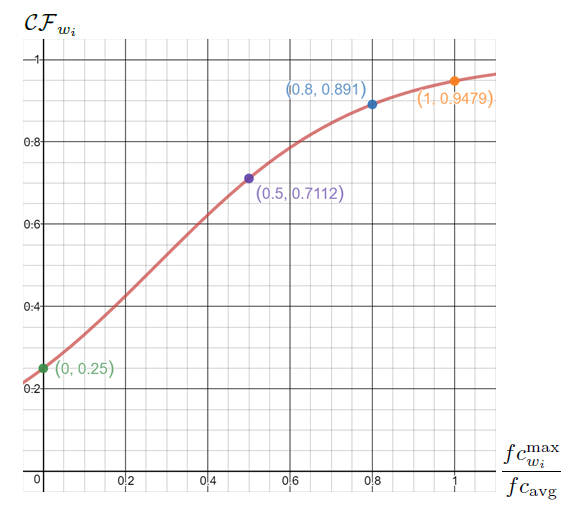
\includegraphics[width=0.6\textwidth]{./figure/conf.png}
\end{figure}
\end{frame}
\begin{frame}
\frametitle{Confidence in general CopeOpi scores}
\begin{figure}
\centering
\caption{An example of $\mathcal{COP}$ and $\mathcal{CF}\text{-}\mathcal{COP}$}
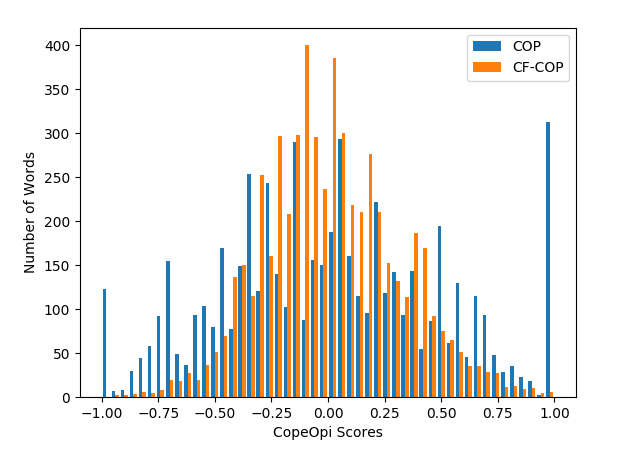
\includegraphics[width=0.7\textwidth]{./figure/conf_SA(EN)(A).png}
\end{figure}
\end{frame}
\subsubsection{What are general CopeOpi Scores?}
\begin{frame}
\frametitle{What are general CopeOpi Scores?}
\begin{itemize}
\item Class-tendency scores of words
	\begin{itemize}
	\item Class-tendencies: be in the class/not be in the class
	\item Strength of class-tendencies
	\item $+1$(be in the class) $\sim$ $-1$(not be in the class)
	\end{itemize}
\item Can be used in languages other than Chinese
	\begin{itemize}
	\item Since we regard words as the basic units
	\end{itemize}
\item Can be used in binary text classification other than sentiment analysis
	\begin{itemize}
	\item Since we take binary annotated documents as context
	\end{itemize}
\end{itemize}
\end{frame}
\subsection{CopeOpi Vectors}
\subsubsection{Motivations for CopeOpi vectors}
\begin{frame}
\frametitle{Motivations for CopeOpi vectors}
\begin{itemize}
\item There are many text classification problems with more than two categories
	\begin{itemize}
	\item But CopeOpi scores can represent at most two classes by as positive or negative
	\end{itemize}
\end{itemize}
\end{frame}
\subsubsection{How to construct CopeOpi vectors?}
\begin{frame}
\frametitle{How to construct CopeOpi vectors?}
\begin{itemize}
\item How do we solve a multi-class classification problem?
	\begin{itemize}
	\item Divide-and-conquer
		\begin{itemize}
		\item Decomposing a multi-class classification problem into many binary classification sub-problems
		\end{itemize}
	\end{itemize}
\item Decomposition strategies\cite{Aly2005multi}
	\begin{itemize}
	\item One-against-all strategy (OAA)
	\item One-against-one strategy (OAO)
	\end{itemize}
\end{itemize}
\end{frame}
\subsubsection{The computation scheme of CopeOpi vectors}
\begin{frame}
\frametitle{The computation scheme of CopeOpi vectors}
\begin{block}{Computation Scheme (CopeOpi Vectors)}
Given $n$ corpora $\mathbb{D}_{c_1},\mathbb{D}_{c_2},\dots,\mathbb{D}_{c_n}$ and the corresponding classes $\mathbb{C}=\{c_1,c_2,\dots,c_n\}$
\begin{itemize}
\item $\mathbb{D}_{c_i}=\{\langle d,c \rangle \where c=c_i\}$
	\begin{itemize}
	\item the vocabulary $\mathbb{V}_{c_i}=\{\text{unique words in }\mathbb{D}_{c_i}\}$
	\end{itemize}
\end{itemize}
For each unique word $w_i \in \cup_{c \in \mathbb{C}} \mathbb{V}_{c}$, we can compute its CopeOpi vector $\overrightarrow{\mathcal{COP}}_{w_i}$ by one of the decomposition strategies.
\end{block}
\end{frame}

\begin{frame}
\frametitle{The computation scheme of CopeOpi vectors}
\begin{block}{Computation Scheme (CopeOpi Vectors)(One-against-all)}
For each class $c_j \in \mathbb{C}$, we can construct two opposite subests
\begin{itemize}
\item the positive set $\mathbb{P}^{c_j}_{w_i} = \{c_j\}$
	\begin{itemize}
		\item the corpus ${\mathbb{D}_\mathbb{P}}^{c_j}_{w_i} = \{\mathbb{D}_{c_j}\}$
		\item the vocabulary ${\mathbb{V}_\mathbb{P}}^{c_j}_{w_i} = \{\mathbb{V}_{c_j}\}$
	\end{itemize}
\item the negative set $\mathbb{N}^{c_j}_{w_i} = \mathbb{C} \setminus \{c_j\}$
	\begin{itemize}
	\item the corpus ${\mathbb{D}_\mathbb{N}}^{c_j}_{w_i} = \{\mathbb{D}_{c} \where c \in \mathbb{N}\}$
	\item the vocabulary ${\mathbb{V}_\mathbb{N}}^{c_j}_{w_i} = \cup_{c \in \mathbb{N}^{c_j}_{w_i}} \mathbb{V}_{c}$
	\end{itemize}
\end{itemize}
and compute its CopeOpi score $\mathcal{COP}^{c_j}_{w_i}$
\end{block}
\end{frame}

\begin{frame}
\frametitle{The computation scheme of CopeOpi vectors}
\begin{block}{Computation Scheme (CopeOpi Vectors)(One-against-all)}
The CopeOpi score $\mathcal{COP}^{c_j}_{w_i}$ of a word $w_i$ with respect to class $c_j$
\begin{equation*}
\begin{gathered}
\mathcal{P}^{c_j}_{w_i} = \dfrac {
	fp^{c_j}_{w_i} \divby \sum_{w \in {\mathbb{V}_\mathbb{P}}^{c_j}_{w_i}} fp^{c_j}_w
}{
	fp^{c_j}_{w_i} \divby \sum_{w \in {\mathbb{V}_\mathbb{P}}^{c_j}_{w_i}} fp^{c_j}_w +
	fn^{c_j}_{w_i} \divby \sum_{w \in {\mathbb{V}_\mathbb{N}}^{c_j}_{w_i}} fn^{c_j}_w
}
\\
\mathcal{N}^{c_j}_{w_i} = \dfrac {
	fn^{c_j}_{w_i} \divby \sum_{w \in {\mathbb{V}_\mathbb{N}}^{c_j}_{w_i}} fn^{c_j}_w
}{
	fp^{c_j}_{w_i} \divby \sum_{w \in {\mathbb{V}_\mathbb{P}}^{c_j}_{w_i}} fp^{c_j}_w +
	fn^{c_j}_{w_i} \divby \sum_{w \in {\mathbb{V}_\mathbb{N}}^{c_j}_{w_i}} fn^{c_j}_w
}
\\
\mathcal{COP}^{c_j}_{w_i} = \mathcal{P}^{c_j}_{w_i} - \mathcal{N}^{c_j}_{w_i}
\end{gathered}
\end{equation*}
\end{block}
\begin{flushright}
\vspace{-9.5ex}
\scalebox{0.7}{
\begin{tabular}{rp{0.5cm}p{0.5cm}}
& ${\mathbb{D}_\mathbb{P}}^{c_j}_{w_i}$ & ${\mathbb{D}_\mathbb{N}}^{c_j}_{w_i}$\\ \cline{2-3} 
\multicolumn{1}{l|}{$w_i$} & \multicolumn{1}{l|}{$fp^{c_j}_{w_i}$} & \multicolumn{1}{l|}{$fn^{c_j}_{w_i}$} \\ \cline{2-3} 
\multicolumn{1}{l|}{} & \multicolumn{1}{l|}{} & \multicolumn{1}{l|}{} \\ \cline{2-3} 
\end{tabular}}
\end{flushright}
\end{frame}

\begin{frame}
\frametitle{The computation scheme of CopeOpi vectors}
\begin{block}{Computation Scheme (CopeOpi Vectors)(One-against-all)}
The CopeOpi vector $\overrightarrow{\mathcal{COP}}_{w_i}$ of word $w_i$ will be composed of these $n$ CopeOpi scores.
\begin{equation*}
\overrightarrow{\mathcal{COP}}_{w_i} = (\mathcal{COP}^{c_1}_{w_i},\mathcal{COP}^{c_2}_{w_i},\dots,\mathcal{COP}^{c_n}_{w_i})
\end{equation*}
\end{block}
\end{frame}

\begin{frame}
\frametitle{The computation scheme of CopeOpi vectors}
\begin{block}{Computation Scheme (CopeOpi Vectors)(One-against-one)}
For each class-pair $c_j,c_k \in \mathbb{C}$, we can construct two opposite subests
\begin{itemize}
\item the positive set $\mathbb{P}^{c_{j,k}}_{w_i} = \{c_j\}$
	\begin{itemize}
	\item the corpus ${\mathbb{D}_\mathbb{P}}^{c_{j,k}}_{w_i} = \{\mathbb{D}_{c_j}\}$
	\item the vocabulary ${\mathbb{V}_\mathbb{P}}^{c_{j,k}}_{w_i} = \{\mathbb{V}_{c_j}\}$
	\end{itemize}
\item the negative set $\mathbb{N}^{c_{j,k}}_{w_i} = \{c_k\}$
	\begin{itemize}
	\item the corpus ${\mathbb{D}_\mathbb{N}}^{c_{j,k}}_{w_i} = \{\mathbb{D}_{c_k}\}$
	\item the vocabulary ${\mathbb{V}_\mathbb{N}}^{c_{j,k}}_{w_i} = \{\mathbb{V}_{c_k}\}$
	\end{itemize}
\end{itemize}
and compute its CopeOpi score $\mathcal{COP}^{c_{j,k}}_{w_i}$
\end{block}
\end{frame}

\begin{frame}
\frametitle{The computation scheme of CopeOpi vectors}
\begin{block}{Computation Scheme (CopeOpi Vectors)(One-against-one)}
The CopeOpi score $\mathcal{COP}^{c_{j,k}}_{w_i}$ of a word $w_i$ with respect to class-pair $c_j,c_k$
\begin{equation*}
\begin{gathered}
\mathcal{P}^{c_{j,k}}_{w_i} = \dfrac {
	fp^{c_{j,k}}_{w_i} \divby \sum_{w \in {\mathbb{V}_\mathbb{P}}^{c_{j,k}}_{w_i}} fp^{c_{j,k}}_w
}{
	fp^{c_{j,k}}_{w_i} \divby \sum_{w \in {\mathbb{V}_\mathbb{P}}^{c_{j,k}}_{w_i}} fp^{c_{j,k}}_w +
	fn^{c_{j,k}}_{w_i} \divby \sum_{w \in {\mathbb{V}_\mathbb{N}}^{c_{j,k}}_{w_i}} fn^{c_{j,k}}_w
}
\\
\mathcal{N}^{c_{j,k}}_{w_i} = \dfrac {
	fn^{c_{j,k}}_{w_i} \divby \sum_{w \in {\mathbb{V}_\mathbb{N}}^{c_{j,k}}_{w_i}} fn^{c_{j,k}}_w
}{
	fp^{c_{j,k}}_{w_i} \divby \sum_{w \in {\mathbb{V}_\mathbb{P}}^{c_{j,k}}_{w_i}} fp^{c_{j,k}}_w +
	fn^{c_{j,k}}_{w_i} \divby \sum_{w \in {\mathbb{V}_\mathbb{N}}^{c_{j,k}}_{w_i}} fn^{c_{j,k}}_w
}
\\
\mathcal{COP}^{c_{j,k}}_{w_i} = \mathcal{P}^{c_{j,k}}_{w_i} - \mathcal{N}^{c_{j,k}}_{w_i}
\end{gathered}
\end{equation*}
\end{block}
\begin{flushright}
\vspace{-9.5ex}
\scalebox{0.7}{
\begin{tabular}{rp{0.5cm}p{0.5cm}}
& ${\mathbb{D}_\mathbb{P}}^{c_{j,k}}_{w_i}$ & ${\mathbb{D}_\mathbb{N}}^{c_{j,k}}_{w_i}$\\ \cline{2-3} 
\multicolumn{1}{l|}{$w_i$} & \multicolumn{1}{l|}{$fp^{c_{j,k}}_{w_i}$} & \multicolumn{1}{l|}{$fn^{c_{j,k}}_{w_i}$} \\ \cline{2-3} 
\multicolumn{1}{l|}{} & \multicolumn{1}{l|}{} & \multicolumn{1}{l|}{} \\ \cline{2-3} 
\end{tabular}}
\end{flushright}
\end{frame}

\begin{frame}
\frametitle{The computation scheme of CopeOpi vectors}
\begin{block}{Computation Scheme (CopeOpi Vectors)(One-against-one)}
The CopeOpi vector $\overrightarrow{\mathcal{COP}}_{w_i}$ of word $w_i$ will be composed of these $\frac{1}{2}n(n-1)$ CopeOpi scores.
\begin{equation*}
\overrightarrow{\mathcal{COP}}_{w_i} = (\mathcal{COP}^{c_{1,2}}_{w_i},\mathcal{COP}^{c_{1,3}}_{w_i},\dots,\mathcal{COP}^{c_{n-1,n}}_{w_i})
\end{equation*}
\end{block}
\end{frame}

\subsubsection{Customized CopeOpi vectors}
\begin{frame}
\frametitle{Customized CopeOpi vectors}
\begin{itemize}
\item OAA and OAO strategies guide the basic construction of CopeOpi vectors for multi-class text classification
\item In general, any subset of classes can be grouped as a positive set or a negative set
	\begin{itemize}
	\item $\mathbb{Q}$-against-$\mathbb{R}$ strategy
	\end{itemize}
\end{itemize}
\end{frame}

\begin{frame}
\frametitle{Customized CopeOpi vectors}
\begin{block}{Computation Scheme (CopeOpi Vectors)($\mathbb{Q}$-against-$\mathbb{R}$)}
For any two subsets of classes $\mathbb{Q},\mathbb{R}$, we can construct two opposite subsets
\begin{itemize}
\item the positive set $\mathbb{P}^{\mathbb{Q},\mathbb{R}}_{w_i} = \mathbb{Q}$
	\begin{itemize}
	\item the corpus ${\mathbb{D}_\mathbb{P}}^{\mathbb{Q},\mathbb{R}}_{w_i} = \{\mathbb{D}_{c} \where c \in \mathbb{Q}\}$
	\item the vocabulary ${\mathbb{V}_\mathbb{P}}^{\mathbb{Q},\mathbb{R}}_{w_i} = \cup_{c \in \mathbb{Q}} \mathbb{V}_{c}$
	\end{itemize}
\item the negative set $\mathbb{N}^{\mathbb{Q},\mathbb{R}}_{w_i} = \mathbb{R}$
	\begin{itemize}
	\item the corpus ${\mathbb{D}_\mathbb{N}}^{\mathbb{Q},\mathbb{R}}_{w_i} = \{\mathbb{D}_{c} \where c \in \mathbb{R}\}$
	\item the vocabulary ${\mathbb{V}_\mathbb{N}}^{\mathbb{Q},\mathbb{R}}_{w_i} = \cup_{c \in \mathbb{R}} \mathbb{V}_{c}$
	\end{itemize}
\end{itemize}
and compute its CopeOpi score $\mathcal{COP}^{\mathbb{Q},\mathbb{R}}_{w_i}$
\end{block}
\end{frame}

\begin{frame}
\frametitle{Customized CopeOpi vectors}
\begin{block}{Computation Scheme (CopeOpi Vectors)($\mathbb{Q}$-against-$\mathbb{R}$)}
The CopeOpi score $\mathcal{COP}^{\mathbb{Q},\mathbb{R}}_{w_i}$ of a word $w_i$ with respect to class subsets $\mathbb{Q},\mathbb{R}$
\begin{equation*}
\begin{gathered}
\mathcal{P}^{\mathbb{Q},\mathbb{R}}_{w_i} = \dfrac {
	fp^{\mathbb{Q},\mathbb{R}}_{w_i} \divby \sum_{w \in {\mathbb{V}_\mathbb{P}}^{\mathbb{Q},\mathbb{R}}_{w_i}} fp^{\mathbb{Q},\mathbb{R}}_w
}{
	fp^{\mathbb{Q},\mathbb{R}}_{w_i} \divby \sum_{w \in {\mathbb{V}_\mathbb{P}}^{\mathbb{Q},\mathbb{R}}_{w_i}} fp^{\mathbb{Q},\mathbb{R}}_w +
	fn^{\mathbb{Q},\mathbb{R}}_{w_i} \divby \sum_{w \in {\mathbb{V}_\mathbb{N}}^{\mathbb{Q},\mathbb{R}}_{w_i}} fn^{\mathbb{Q},\mathbb{R}}_w
}
\\
\mathcal{N}^{\mathbb{Q},\mathbb{R}}_{w_i} = \dfrac {
	fn^{\mathbb{Q},\mathbb{R}}_{w_i} \divby \sum_{w \in {\mathbb{V}_\mathbb{N}}^{\mathbb{Q},\mathbb{R}}_{w_i}} fn^{\mathbb{Q},\mathbb{R}}_w
}{
	fp^{\mathbb{Q},\mathbb{R}}_{w_i} \divby \sum_{w \in {\mathbb{V}_\mathbb{P}}^{\mathbb{Q},\mathbb{R}}_{w_i}} fp^{\mathbb{Q},\mathbb{R}}_w +
	fn^{\mathbb{Q},\mathbb{R}}_{w_i} \divby \sum_{w \in {\mathbb{V}_\mathbb{N}}^{\mathbb{Q},\mathbb{R}}_{w_i}} fn^{\mathbb{Q},\mathbb{R}}_w
}
\\
\mathcal{COP}^{\mathbb{Q},\mathbb{R}}_{w_i} = \mathcal{P}^{\mathbb{Q},\mathbb{R}}_{w_i} - \mathcal{N}^{\mathbb{Q},\mathbb{R}}_{w_i}
\end{gathered}
\end{equation*}
\end{block}
\begin{flushright}
\vspace{-9.5ex}
\scalebox{0.7}{
\begin{tabular}{rp{0.5cm}p{0.5cm}}
& ${\mathbb{D}_\mathbb{P}}^{\mathbb{Q},\mathbb{R}}_{w_i}$ & ${\mathbb{D}_\mathbb{N}}^{\mathbb{Q},\mathbb{R}}_{w_i}$\\ \cline{2-3} 
\multicolumn{1}{l|}{$w_i$} & \multicolumn{1}{l|}{$fp^{\mathbb{Q},\mathbb{R}}_{w_i}$} & \multicolumn{1}{l|}{$fn^{\mathbb{Q},\mathbb{R}}_{w_i}$} \\ \cline{2-3} 
\multicolumn{1}{l|}{} & \multicolumn{1}{l|}{} & \multicolumn{1}{l|}{} \\ \cline{2-3} 
\end{tabular}}
\end{flushright}
\end{frame}

\subsubsection{What are CopeOpi vectors?}
\begin{frame}
\frametitle{What are CopeOpi vectors?}
\begin{itemize}
\item Word vectors, whose elements are classes-tendencies scores
	\begin{itemize}
	\item Classes-tendencies: be in the classes/not be in the classes
	\item Strength of classes-tendencies
	\item $+1$(be in the classes) $\sim$ $-1$(not be in the classes)
	\end{itemize}
\item Can be used in multi-class text classification
\end{itemize}
\end{frame}


\section{Experiments}
\begin{frame}{Experiments}
To verify the functionality of CopeOpi vectors, we make comparisons with several commonly used features of text, and examine these features on different types of classifiers to solve text classification problems
\begin{itemize}
\item Types
	\begin{itemize}
	\item Sentiment analysis (SA)
	\item Topic categorization (TC)
	\end{itemize}
\item Languages
	\begin{itemize}
	\item English (EN)
	\item Chinese (ZH)
	\end{itemize}
\end{itemize}
\end{frame}

\subsection{Flowchart and Settings}
\begin{frame}{Flowchart}
	\begin{figure}
	\centering
	\caption{Flowchart of experiments}
	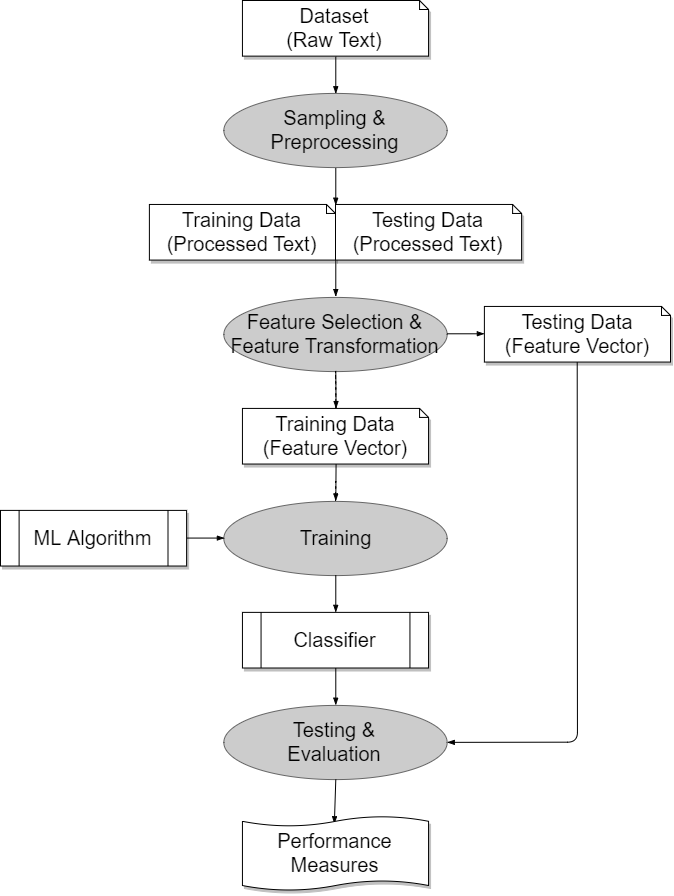
\includegraphics[width=0.48\textwidth]{./figure/flowchart.png}
	\end{figure}
\end{frame}

\subsubsection{Sampling and Preprocessing}
\begin{frame}{Sampling and Preprocessing}
	\begin{itemize}
	\item Sampling
		\begin{itemize}
			\item A training set
			\item A testing set
		\end{itemize}
	\item Preprocessing: unified procedure for each language
		\begin{itemize}
			\item For English: tokenizing, stripping tags, stripping punctuations, stripping multiple whitespaces, stripping numeric, removing stopwords, stripping shorts and stemming
			\item For Chinese: word segmentation and remove characters that are outside UTF-8 \texttt{[\textbackslash u4E00-\textbackslash u9FFF]}.
		\end{itemize}
	\end{itemize}
\end{frame}

\subsubsection{Feature Selection and Feature Transformation}
\begin{frame}{Feature Selection and Feature Transformation}
	\begin{itemize}
	\item Term-document matrix models
		\begin{itemize}
		\item BoW and its LSA-truncated version BoW(LSA)
			\begin{itemize}
			\item Bag-of-word
			\end{itemize}
		\item TF-IDF and its LSA-truncated version TF-IDF(LSA)
			\begin{itemize}
			\item $TF(w_i,d_j) = f{d_j}_{w_i} \divby \sum_{w \in d_j} f{d_j}_{w_i}$
			\item[] $IDF_{w_i} = \log \frac{|\mathbb{D}|}{|\{j:w_i \in d_j\}|}$
			\item[] $TF\text{-}IDF(w_i,d_j) = TF(w_i,d_j) \times IDF_{w_i}$
			\end{itemize}
		\end{itemize}
	\item Word-context matrix models
		\begin{itemize}
		\item Word2vec\cite{Mikolov2013ord2vec} and its extension Doc2vec\cite{le2014doc2vec}
		\item GolVe\cite{Pennington2014glove}
			\begin{itemize}
			\item Neural language models
			\end{itemize}
		\end{itemize}
	\end{itemize}
\end{frame}

\subsubsection{Training Classifiers}
\begin{frame}{Training Classifiers}
	\begin{itemize}
	\item k-nearest neighbor classifiers (kNN)
	\item Naive Bayes classifiers (NB)
		\begin{itemize}
		\item Multinomial distribution: BoW, TF-IDF
		\item Gaussian distribution: others
		\end{itemize}
	\item Logistic regression classifiers (LR)
	\item Support vector machines (SVM)
		\begin{itemize}
		\item Linear kernel
		\end{itemize}
	\item Neural networks (NN)
		\begin{itemize}
		\item One hidden layer with size 100
		\end{itemize}
	\end{itemize}
\end{frame}

\subsubsection{Testing and Evaluation}
\begin{frame}{Testing and Evaluation}
	\begin{itemize}
	\item Precision, recall, F1-scores for binary classification
		\begin{itemize}
		\item $Presision_c = TP_c \divby (TP_c+FP_c)$
		\item[] $Recall_c = TP_c \divby (TP_c+FN_c)$
		\item[] $F1_c = (2 \times Presision_c \times Recall_c) \divby (Presision_c+Recall_c)$
		\end{itemize}
	\item Macro-F1 for multi-class classification
		\begin{itemize}
		\item $Macro\text{-}F1 = \frac{1}{|\mathbb{C}|} \sum_{c \in \mathbb{C}} F1_c$
		\end{itemize}
	\end{itemize}
	\begin{table}[h]
\centering
\caption{The contingency table of binary classification}
\label{tab:f1}
\begin{tabular}{ll|c|c|}
\hline
\multicolumn{2}{|l|}{\multirow{2}{*}{}}                        & \multicolumn{2}{c|}{Real}           \\ \cline{3-4} 
\multicolumn{2}{|l|}{}                                         & True                & False               \\ \hline
\multicolumn{1}{|c|}{\multirow{2}{*}{Predicted}} & True  & True positive (TP)  & False positive (FP) \\ \cline{2-4} 
\multicolumn{1}{|c|}{}                                 & False & False negative (FN) & True negative (TN)  \\ \hline
\end{tabular}
\end{table}
\end{frame}

\subsection{Experiments: Sentiment Analysis}
\subsubsection{Datasets}
\begin{frame}
\frametitle{Datasets}
	\begin{itemize}
	\item Both are 5-star integer ratings
		\begin{itemize}
		\item $+5$(positive) $\sim$ $+1$(negative)
		\end{itemize}
	\end{itemize}
\vspace{-4ex}
\begin{table}[]
\centering
\caption{Sentiment analysis datasets}
\label{tab:sa_data}
\begin{tabular}{|l|c|m{0.3\textwidth}|c|c|}
\hline
Name      & Language & \multicolumn{1}{c|}{Description}
              & \multicolumn{1}{c|}{Source} \\ \hline
Yelp Dataset\cite{Yelp9} & English           & Customer reviews about local business such as restaurants, hair stylists, mechanics, etc.
                                  & Yelp \\ \hline
MioChnCorp\cite{MioChnCorp}   & Chinese           & Customer reviews about hotels.
                          & Dianping \\ \hline
\end{tabular}
\end{table}
\end{frame}

\subsubsection{Experiments Datasets}
\begin{frame}
\frametitle{Experiments Datasets}
	\begin{itemize}
	\item 15000 samples
	\item Train-test-split 0.5/0.5
	\item Balanced
	\end{itemize}
\begin{table}[]
\centering
\caption{Sentiment analysis experiments datasets}
\begin{tabular}{|c|c|c|c|c|c|}
\hline
     & Rating-1      & Rating-2      & Rating-3 & Rating-4      & Rating-5      \\ \hline
SA(A)(2) & \multicolumn{2}{c|}{Negative} &          & \multicolumn{2}{c|}{Positive} \\ \hline
SA(B)(3) & Negative      &               & Neutral  &               & Positive      \\ \hline
SA(C)(5) & Rating-1      & Rating-2      & Rating-3 & Rating-4      & Rating-5      \\ \hline
\end{tabular}
\end{table}
\end{frame}

\subsubsection{Results and Observations}
\begin{frame}
\frametitle{Results and Observations 1}
	\vspace{\expfigvspace}
	\begin{figure}
	\centering
	\caption{F1-score of SA(EN)(A)}
	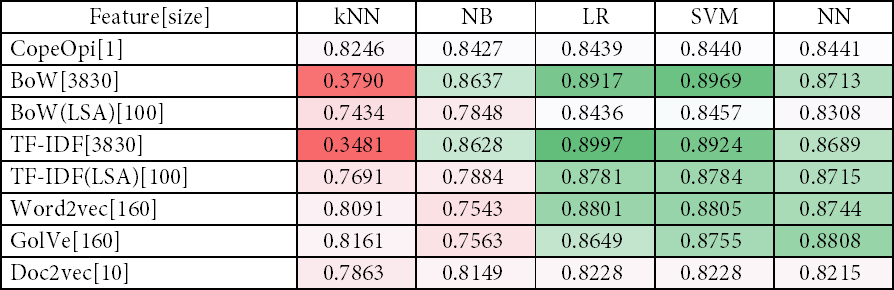
\includegraphics[width=0.75\textwidth]{./figure/01A1.png}
	\caption{F1-score of SA(ZH)(A)}
	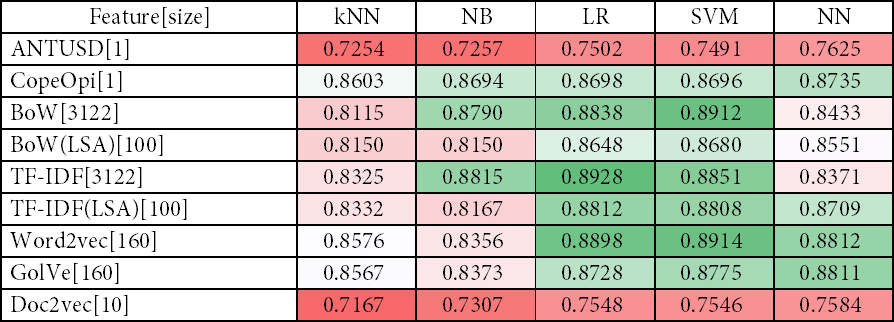
\includegraphics[width=0.75\textwidth]{./figure/02A1.png}
	\end{figure}
\end{frame}
\begin{frame}
\frametitle{Results and Observations 1}
	\begin{itemize}
	\item SA(A)
		\begin{itemize}
		\item Binary text classification
		\item CopeOpi = general CopeOpi scores
		\end{itemize}
	\item Compare the best F1-score of CopeOpi and the best F1-score of each experiment
		\begin{itemize}
		\item Lose by 5.56\% in SA(EN)
		\item Lose by 1.93\% in SA(ZH)
		\end{itemize}
	\item This shows that the computation scheme of general CopeOpi scores is feasible
	\end{itemize}
\end{frame}

\begin{frame}
\frametitle{Results and Observations 2}
	\begin{figure}
	\centering
	\caption{F1-score of SA(ZH)(A)}
	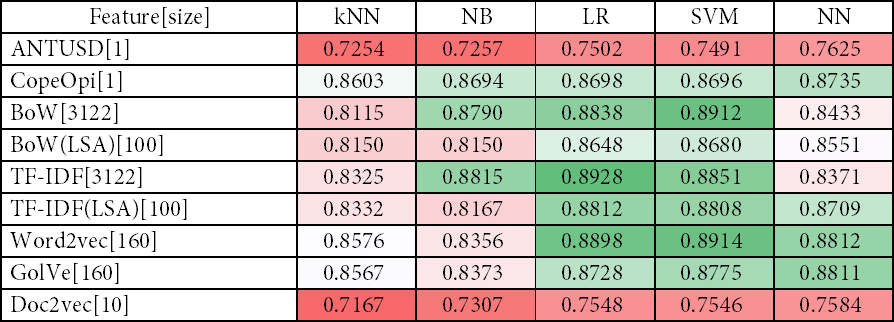
\includegraphics[width=0.8\textwidth]{./figure/02A1.png}
	\end{figure}
\end{frame}
\begin{frame}
\frametitle{Results and Observations 2}
	\begin{itemize}
	\item SA(ZH)(A)
		\begin{itemize}
		\item CopeOpi scores in ANTUSD
		\end{itemize}
	\item Compare the F1-scores of CopeOpi and the F1-scores of ANTUSD
		\begin{itemize}
		\item Outperform by more than 10\%
		\end{itemize}
	\item This shows general CopeOpi scores function normally without manually filtering non-opinion words and are more applicable to the dataset
	\end{itemize}
\end{frame}

\begin{frame}
\frametitle{Results and Observations 3}
	\vspace{\expfigvspace}
	\begin{figure}
	\centering
	\caption{F1-score of SA(EN)(B)}
	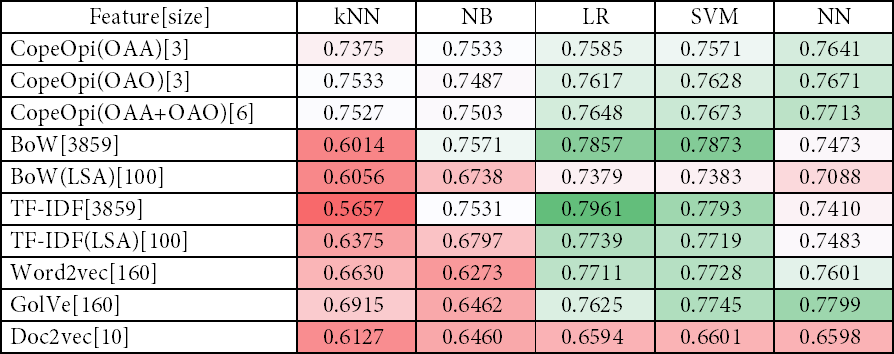
\includegraphics[width=0.75\textwidth]{./figure/01A2.png}
	\caption{F1-score of SA(ZH)(B)}
	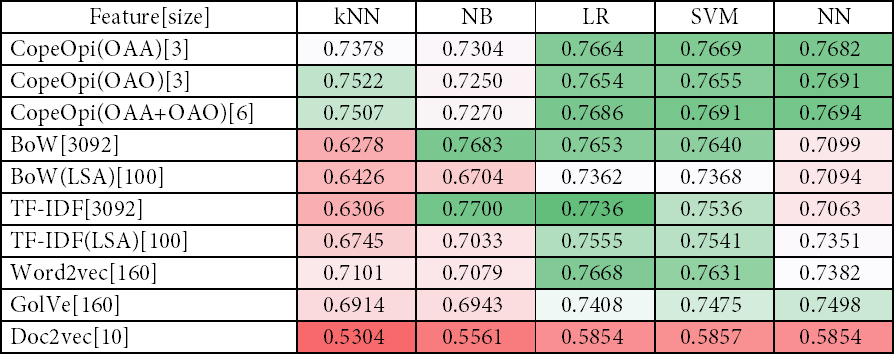
\includegraphics[width=0.75\textwidth]{./figure/02A2.png}
	\end{figure}
\end{frame}
\begin{frame}
\frametitle{Results and Observations 3}
	\vspace{\expfigvspace}
	\begin{figure}
	\centering
	\caption{F1-score of SA(EN)(C)}
	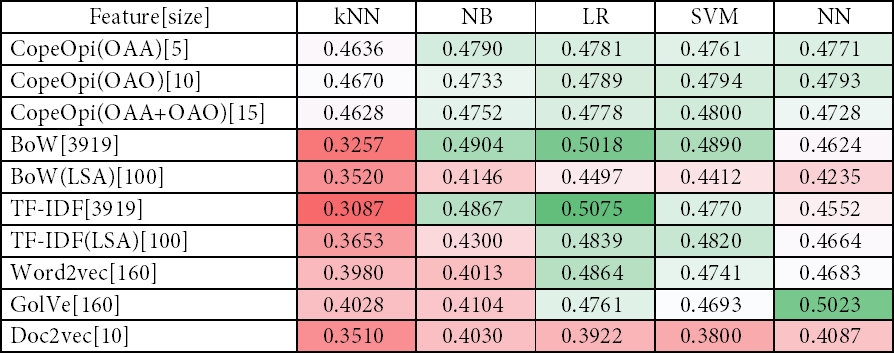
\includegraphics[width=0.75\textwidth]{./figure/01A3.png}
	\caption{F1-score of SA(ZH)(C)}
	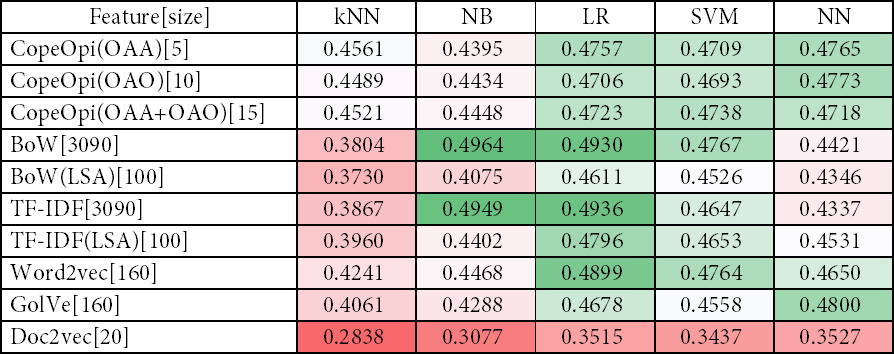
\includegraphics[width=0.75\textwidth]{./figure/02A3.png}
	\end{figure}
\end{frame}
\begin{frame}
\frametitle{Results and Observations 3}
	\begin{itemize}
	\item SA(B), SA(C)
		\begin{itemize}
		\item Multi-class text classification
		\item CopeOpi = CopeOpi vectors
		\end{itemize}
	\item Compare the F1-scores of CopeOpi and the F1-scores of each experiment
		\begin{itemize}
		\item Lose by 2.49\% in SA(EN)(B)
		\item Lose by 2.79\% in SA(EN)(C)
		\item Lose by 0.42\% in SA(ZH)(B)
		\item Lose by 1.92\% in SA(ZH)(C)
		\end{itemize}
	\item This shows that the computation scheme of CopeOpi vectors is feasible
	\end{itemize}
\end{frame}

\begin{frame}
\frametitle{Results and Observations 4}
	\begin{itemize}
	\item SA(A)
		\begin{itemize}
		\item Binary text classification
		\item CopeOpi = general CopeOpi scores
		\item In 2/10 exps for each classifier, the F1-scores of CopeOpi are better than the average F1-score
		\end{itemize}
	\item SA(B), SA(C)
		\begin{itemize}
		\item Multi-class text classification
		\item CopeOpi = CopeOpi vectors
		\item In 20/20 exps for each classifier, the F1-scores of CopeOpi are better than the average F1-score of each classifier
		\end{itemize}
	\item This shows that CopeOpi vectors in multi-class text classification is more effective then CopeOpi scores in binary text classification
	\end{itemize}
\end{frame}

\subsection{Experiments: Topic Categorization}
\subsubsection{Datasets}
\begin{frame}
\frametitle{Datasets}
	\begin{itemize}
	\item Both are 20 classes
	\end{itemize}
\begin{table}[h]
\footnotesize
\centering
\caption{Topic categorization datasets}
\label{tab:tc_data}
\begin{tabular}{|l|c|c|c|c|}
	\hline
	\multicolumn{1}{|c|}{Dataset} & Language & \# of Classes & Balanced & Train:Test \\ \hline
	20 Newsgroup                  & English  & 20            & Yes      & 0.6:0.4    \\ \hline
	Fudan University TC Corpus    & Chinese  & 20            & No       & 0.5:0.5    \\ \hline
\end{tabular}
\end{table}
\subsubsection{Experiments Datasets}
\end{frame}
\begin{frame}
\frametitle{Experiments Datasets}
	\begin{itemize}
	\item TC(EN) train-test-split 0.6/0.4
	\item TC(ZH) train-test-split 0.5/0.5
	\end{itemize}
\begin{table}[h]
\footnotesize
\centering
\begin{minipage}{\textwidth}
\caption{Topic categorization experiments datasets}
\label{tab:tc_dataexp}
\begin{subtable}{0.58\textwidth}
\centering
\caption{Sampling of TC(EN)}
\scalebox{0.72}{
\begin{tabular}{|l|c|c|c|c|}
	\hline
	\multicolumn{1}{|c|}{Classes} & (A)        & (B)                        & (C)       & (D)       \\ \hline
	alt.atheism                   & 480:319    & 480:319                    &           &           \\ \hline
	comp.graphics                 & 584:389    & \multirow{5}{*}{2936:1955} & 584:389   &           \\ \cline{1-2} \cline{4-5} 
	comp.os.ms-windows.misc       & 591:394    &                            & 591:394   &           \\ \cline{1-2} \cline{4-5} 
	comp.sys.ibm.pc.hardware      & 590:392    &                            & 590:392   &           \\ \cline{1-2} \cline{4-5} 
	comp.sys.mac.hardware         & 578:385    &                            & 578:385   &           \\ \cline{1-2} \cline{4-5} 
	comp.windows.x                & 593:395    &                            & 593:395   &           \\ \hline
	misc.forsale                  & 585:390    & 585:390                    &           &           \\ \hline
	rec.autos                     & 594:396    & \multirow{4}{*}{2389:1590} &           &           \\ \cline{1-2} \cline{4-5}
	rec.motorcycles               & 598:398    &                            &           &           \\ \cline{1-2} \cline{4-5} 
	rec.sport.baseball            & 597:397    &                            &           &           \\ \cline{1-2} \cline{4-5} 
	rec.sport.hockey              & 600:399    &                            &           &           \\ \hline
	sci.crypt                     & 595:396    & \multirow{4}{*}{2373:1579} &           &           \\ \cline{1-2} \cline{4-5} 
	sci.electronics               & 591:393    &                            &           &           \\ \cline{1-2} \cline{4-5} 
	sci.med                       & 594:396    &                            &           &           \\ \cline{1-2} \cline{4-5} 
	sci.space                     & 593:394    &                            &           &           \\ \hline
	soc.religion.christian        & 599:398    & 599:398                    &           &           \\ \hline
	talk.politics.guns            & 546:364    & \multirow{4}{*}{1952:1301} &           & 546:364   \\ \cline{1-2} \cline{4-5}
	talk.politics.mideast         & 564:376    &                            &           & 564:376   \\ \cline{1-2} \cline{4-5}
	talk.politics.misc            & 465:310    &                            &           & 465:310   \\ \cline{1-2} \cline{4-5}
	talk.religion.misc            & 377:251    &                            &           & 377:251   \\ \hline
	\multicolumn{1}{|c|}{Total}   & 11314:7532 & 11314:7532                 & 2936:1955 & 1952:1301 \\ \hline
\end{tabular}}
\end{subtable}
\begin{subtable}{0.42\textwidth}
\centering
\caption{Sampling of TC(ZH)}
\scalebox{0.72}{
\begin{tabular}{|l|c|c|c|}
	\hline
	\multicolumn{1}{|c|}{Classes} & (A)       & (B)       & (C)     \\ \hline
	Art                           & 740:742   & 740:742   &         \\ \hline
	Literature                    & 33:34     &           & 33:34   \\ \cline{1-2} \cline{3-4}
	Education                     & 59:61     &           & 59:61   \\ \cline{1-2} \cline{3-4}
	Philosophy                    & 44:45     &           & 44:45   \\ \cline{1-2} \cline{3-4}
	History                       & 466:468   & 466:468   &         \\ \cline{1-2} \cline{3-4}
	Space                         & 640:642   & 640:642   &         \\ \hline
	Energy                        & 32:33     &           & 32:33   \\ \hline
	Electronics                   & 27:28     &           & 27:28   \\ \cline{1-2} \cline{3-4}
	Communication                 & 25:27     &           & 25:27   \\ \cline{1-2} \cline{3-4}
	Computer                      & 1357:1358 & 1357:1358 &         \\ \cline{1-2} \cline{3-4}
	Mine                          & 33:34     &           & 33:34   \\ \hline
	Transport                     & 57:59     &           & 57:59   \\ \cline{1-2} \cline{3-4}
	Environment                   & 1217:1218 & 1217:1218 &         \\ \cline{1-2} \cline{3-4}
	Agriculture                   & 1021:1022 & 1021:1022 &         \\ \cline{1-2} \cline{3-4}
	Economy                       & 1600:1601 & 1600:1601 &         \\ \hline
	Law                           & 51:52     &           & 51:52   \\ \hline
	Medical                       & 51:53     &           & 51:53   \\ \cline{1-2} \cline{3-4}
	Military                      & 74:76     &           & 74:76   \\ \cline{1-2} \cline{3-4}
	Politics                      & 1024:1026 & 1024:1026 &         \\ \cline{1-2} \cline{3-4}
	Sports                        & 1253:1254 & 1253:1254 &         \\ \hline
	\multicolumn{1}{|c|}{Total}   & 9804:9833 & 9318:9331 & 486:502 \\ \hline
\end{tabular}}
\end{subtable}
\end{minipage}
\end{table}
\end{frame}
\subsubsection{Results and Observations}

\begin{frame}
\frametitle{Results and Observations 1a}
	\vspace{\expfigvspace}
	\begin{figure}
	\centering
	\caption{F1-score of TC(EN)(A)}
	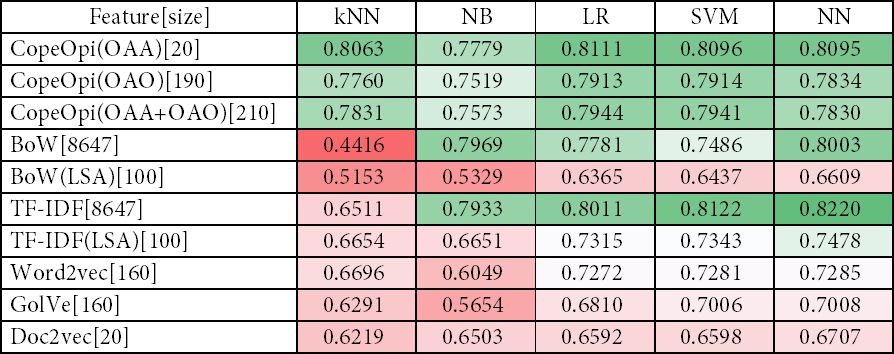
\includegraphics[width=0.75\textwidth]{./figure/01B1.png}
	\caption{F1-score of TC(ZH)(A)}
	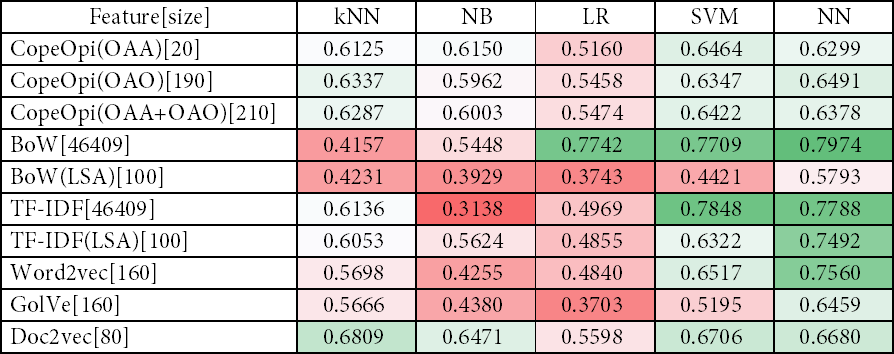
\includegraphics[width=0.75\textwidth]{./figure/02B1.png}
	\end{figure}
\end{frame}
\begin{frame}
\frametitle{Results and Observations 1a}
	\begin{itemize}
	\item TC(EN)(A), TC(ZH)(A)
		\begin{itemize}
		\item Both corpora contain 20 categories
		\end{itemize}
	\item Compare the best F1-score of CopeOpi and the best F1-score of each experiment
		\begin{itemize}
		\item Lose by 1.10\% in TC(EN)(A)
		\item Lose by 14.83\% in TC(ZH)(A)
		\end{itemize}
	\item Considering
		\begin{itemize}
		\item The results of SA shows that CopeOpi performs better in Chinese corpus than in English corpus
		\item The preprocessing procedures are unified for each language
		\end{itemize}
	\item The bad results of TC(ZH)(A) should caused by corpus itself rather than properties of language
or preprocessing	
		\begin{itemize}
		\item Except languages, the biggest difference between their corpus is the balance
		\item CopeOpi can not function well in unbalanced corpora ?
		\end{itemize}
	\end{itemize}
\end{frame}

\begin{frame}
\frametitle{Results and Observations 1b}
	\vspace{\expfigvspace}
	\begin{figure}
	\centering
	\caption{F1-score of TC(EN)(B)}
	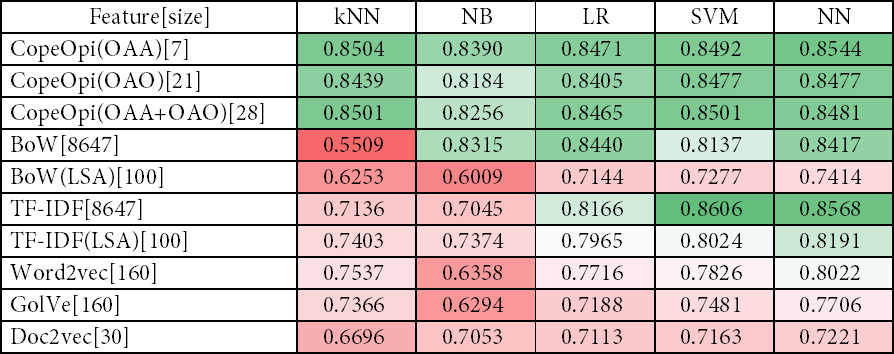
\includegraphics[width=0.75\textwidth]{./figure/01B2.png}
	\caption{F1-score of TC(ZH)(A)}
	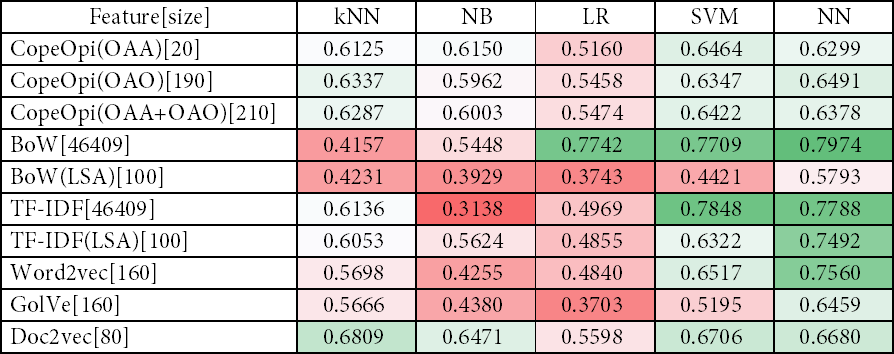
\includegraphics[width=0.75\textwidth]{./figure/02B1.png}
	\end{figure}
\end{frame}
\begin{frame}
\frametitle{Results and Observations 1b}
	\begin{itemize}
	\item TC(EN)(B), TC(ZH)(A)
		\begin{itemize}
		\item Both corpora are unbalanced
		\end{itemize}
	\item Compare the best F1-score of CopeOpi and the best F1-score of each experiment
		\begin{itemize}
		\item Lose by 0.62\% in TC(EN)(B)
		\item Lose by 14.83\% in TC(ZH)(A)
		\end{itemize}
	\item CopeOpi functions as well as usual in one of them
		\begin{itemize}
		\item Except languages, the biggest difference between their corpus is that some of the categories of TC(ZH)(A) have only a few samples
		\end{itemize}
	\item We deduce that The bad results of TC(ZH)(A) should caused by the small-sized categories, not the unbalanced corpus
		\begin{itemize}
		\item CopeOpi can not function well in corpora with small-sized categories
		\end{itemize}
	\end{itemize}
\end{frame}

\begin{frame}
\frametitle{Results and Observations 2}
	\vspace{\expfigvspace}
	\begin{figure}
	\centering
	\caption{F1-score of TC(ZH)(B)}
	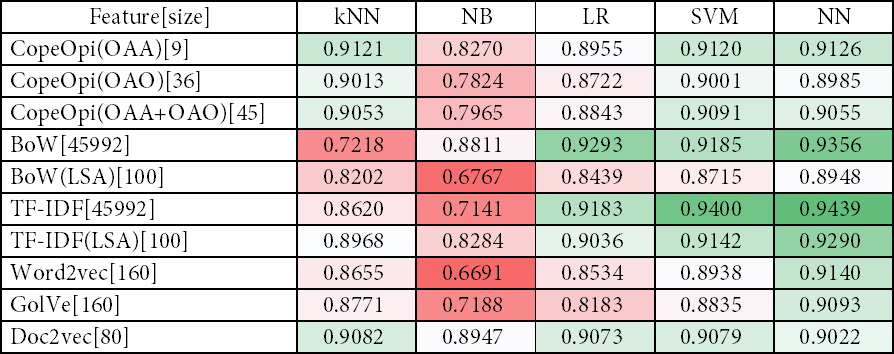
\includegraphics[width=0.75\textwidth]{./figure/02B2.png}
	\caption{F1-score of TC(ZH)(C)}
	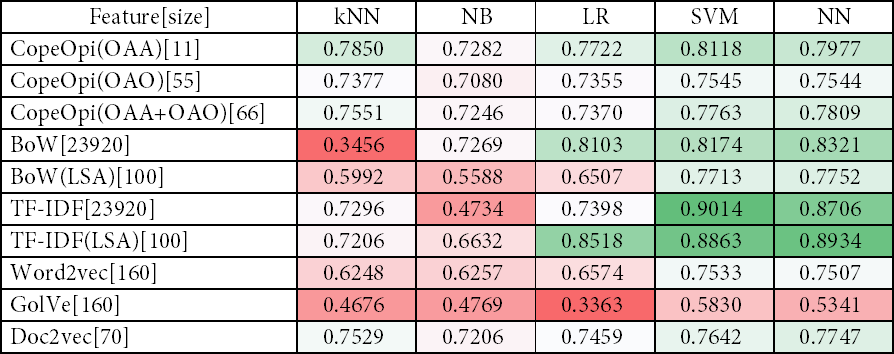
\includegraphics[width=0.75\textwidth]{./figure/02B3.png}
	\end{figure}
\end{frame}
\begin{frame}
\frametitle{Results and Observations 2}
	\begin{itemize}
	\item TC(ZH)(B), TC(ZH)(C)
		\begin{itemize}
		\item The corpus of TC(ZH)(C) is constituted by the corpus of the small-sized categories
		\item The corpus of TC(ZH)(B) is constituted by the corpus of the rest categories
		\end{itemize}
	\item Compare the best F1-score of CopeOpi and the best F1-score of each experiment
		\begin{itemize}
		\item Lose by 3.12\% in TC(ZH)(B)
		\item Lose by 8.95\% in TC(ZH)(C)
		\end{itemize}
	\item This confirms that CopeOpi can not function well in corpora with small-sized categories
	\end{itemize}
\end{frame}

\begin{frame}
\frametitle{Results and Observations 3}
	\vspace{\expfigvspace}
	\begin{figure}
	\centering
	\caption{F1-score of TC(EN)(C)}
	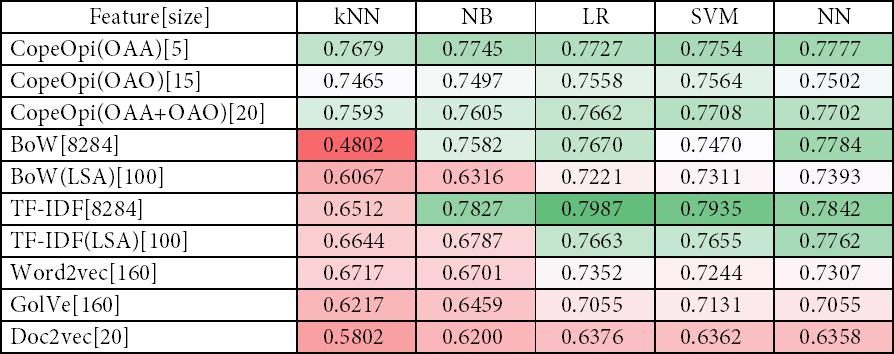
\includegraphics[width=0.75\textwidth]{./figure/01B3.png}
	\caption{F1-score of TC(EN)(D)}
	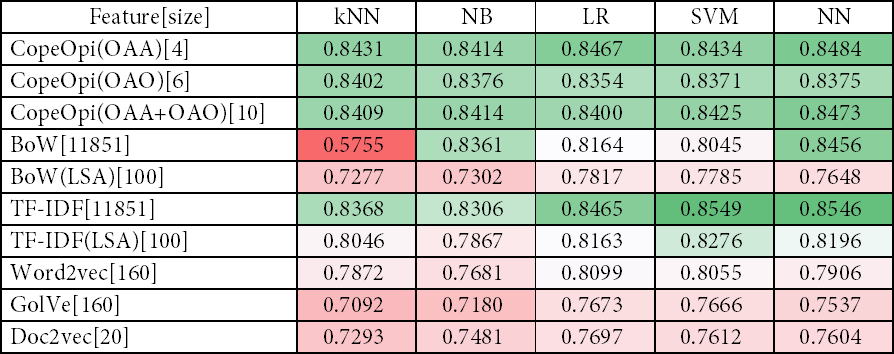
\includegraphics[width=0.75\textwidth]{./figure/01B4.png}
	\end{figure}
\end{frame}
\begin{frame}
\frametitle{Results and Observations 3}
	\begin{itemize}
	\item TC(EN)(C), TC(EN)(D)
		\begin{itemize}
		\item Both corpora are constituted by the corpus with similar categories
		\end{itemize}
	\item Compare the best F1-score of CopeOpi and the best F1-score of each experiment
		\begin{itemize}
		\item Lose by 2.11\% in TC(EN)(C)
		\item Lose by 0.66\% in TC(EN)(D)
		\end{itemize}
	\item This shows that CopeOpi can function well even if the categories are similar
	\end{itemize}
\end{frame}

\subsection{Summary}
\begin{frame}
\frametitle{Summary 1}
	\begin{itemize}
	\item CopeOpi can produce comparable results with a smaller vector size and shorter training time
		\begin{itemize}
		\item In 53/55 exps for each classier, the best F1-score of CopeOpi vectors in multi-class is better than the average F1-score
		\item In 63/65 exps for each classier, the training time of CopeOpi is the shortest
		\item In all exps, the vector size of CopeOpi(OAA) is the smallest
		\end{itemize}
	\end{itemize}
\end{frame}

\begin{frame}
\frametitle{Summary 2}
	\begin{itemize}
	\item Compared to the other features, CopeOpi provides stabler results than the others when applied to
different types of classifiers
		\begin{itemize}
		\item There are some results deviating, but in those cases the deviations are general phenomena for most of features
		\end{itemize}
	\end{itemize}
\end{frame}

\begin{frame}
\frametitle{Summary 3}
	\begin{itemize}
	\item Compared to the winners in multi-class text classification
		\begin{itemize}
		\item Either BoW or TF-IDF
		\item Eexcept the experiments whose corpus has small-sized categories, the difference of the best F1-score of CopeOpi and their F1-score of each experiments is at most 3.12\%
		\end{itemize}
	\item However, the training processes of BoW and TF-IDF cost most in terms of memory space and times
		\begin{itemize}
		\item In 64/65 exps for each classier, the best F1-score of CopeOpi is better than the F1-score of BoW(LSA)[100]
		\item In 50/65 exps for each classier, the best F1-score of CopeOpi is better than the F1-score of TF-IDF(LSA)[100]
		\end{itemize}
	\item Since the vector sizes of BoW and TF-IDF are
related to the number of vocabularies in corpora, in the cases with large corpora, CopeOpi will have
advantages in its efficiency.
	\end{itemize}
\end{frame}
\section{Conclusions and Future Works}
\subsection{Conclusions}
\begin{frame}
\frametitle{Conclusions}
	\begin{itemize}
	\item We propose a vector space model, the word vectors---CopeOpi vectors
		\begin{itemize}
		\item From CopeOpi scores used in Chinese sentiment analysis
		\item To CopeOpi vectors which can be used in multi-class text classification without being limited to languages
		\end{itemize}
	\item We verify the effectiveness and efficiency of CopeOpi vectors by making comparisons with several commonly-used features for text classification
		\begin{itemize}
		\item Various text classification problems in both English and Chinese 
		\item The results show that CopeOpi can produce comparable results with a smaller vector size and shorter training time
		\end{itemize}
	\item In general, CopeOpi vectors are effective and efficient features for multi-class text classification
	\end{itemize}
\end{frame}

\subsection{Future Works}
\begin{frame}
\frametitle{Future Works}
	\begin{enumerate}
	\item More careful term-weighting schemes
		\begin{itemize}
		\item The original CopeOpi scores are computed from dictionaries
			\begin{itemize}
			\item The term-weighting scheme of the current formula $fc \divby \sum_{w}fc_w$
			\end{itemize}					
		 \item But now we compute CopeOpi from nature language corpora
		 	\begin{itemize}
			\item There may be a lot of unrelated words
			\item CopeOpi needs a more careful term-weighting scheme
			\end{itemize}
		\end{itemize}
	\item Strategies to customize CopeOpi vectors
		\begin{itemize}
		\item The number of classes-pairs are exponential to the number of class
			\begin{itemize}
			\item Flexibility
			\item Difficulty
			\end{itemize}
		\end{itemize}
	\end{enumerate}
\end{frame}

\begin{frame}[allowframebreaks]
	\frametitle{References}
	\bibliographystyle{ieeetr}
	\bibliography{ref}
\end{frame}
\end{document}